\documentclass[../main.tex]{subfiles}

\begin{document}

    \section{Méthode} % (fold)
    \label{sec:Méthode}
    Afin de pouvoir résoudre ce problème, il faudra définir un encodage
    spécifique pour représenter un état sur un ordinateur quantique.
    Considérons un encodage d'un spin sur un qubit, soit $\ket{0}\equiv
    \ket{\downarrow}, \ket{1}\equiv\ket{\uparrow}$. Cette façon d'encoder le
    réseau dans l'ordinateur quantique permet d'avoir autant de spins que de
    qubits, soit $N=12$ au maximum ici. Un état général $\ket{\psi}$ peut être
    décrit par $2^N$ paramètres, ce qui est un peu trop compliqué à minimiser.
    Il faudra donc restreindre le nombre de paramètres à ceux qui ont le plus
    d'importance physiquement, afin d'avoir la meilleure borne supérieure possible.

    \subsection{\textit{Variationnal Quantum Eigensolver (VQE)}} % (fold)
    \label{ssub:vqe}
        La VQE (Diagonalisation Quantique Variationnelle) est un algorithme
        variationnel permettant l'estimation de la plus petite valeur propre
        d'un hamiltonien. Cette technique repose sur le principe variationnel,
        en calculant la valeur moyenne de l'hamiltonien en fonction de paramètres,
        qu'on varie afin d'obtenir la valeur minimale.
        \begin{figure}[H]
            \begin{center}
                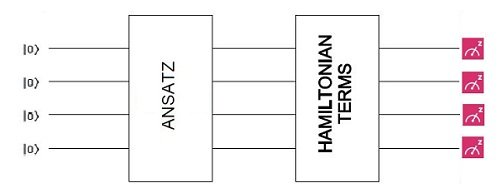
\includegraphics[width=0.95\textwidth]{figs/Schematic-of-quantum-circuit-used-for-VQE-Ansatz-is-created-by-using-different.png}
            \end{center}
            \caption{Schéma conceptuel de la VQE (figure prise de \cite{fig_vqe}).}
            \label{fig:vqe}
        \end{figure}
        Trois morceaux importants figurent dans cet algorithme: l'état d'essai,
        les termes de l'hamiltonien et la fonction d'optimisation. Ce travail
        ne s'intéressait pas aux différentes techniques de minimisation de
        fonctions à plusieurs variables, mais une bonne exploration du domaine
        de l'état d'essai assure de trouver le bon minimum d'énergie associé
        à cet état.\\
        Tout d'abord, il faut encoder l'hamiltonien dans un circuit quantique.
        Or, un hamiltonien général n'est pas unitaire; une propriété fondamentale
        des portes quantiques. Il est tout de fois possible d'effectuer une série
        de mesures qui permettent le calcul de la valeur moyenne de l'énergie.
        On peut décomposer l'hamiltonien sous forme de somme de valeurs moyenne
        d'opérateurs qui s'écrivent complètement sous forme de chaines de matrice de Pauli.
        Il est simple de mesurer les valeurs moyennes de ces chaines de Pauli, comme
        les valeurs moyennes des matrices de Pauli sont simple, voir la figure (\ref{fig:mes}).
        Il suffit de mesurer les qubits dans la base associée à l'opérateur voulu.
        La valeur moyenne de l'opérateur s'obtient ensuite en calculant la moyenne
        pondérée du résultat obtenu.
        \begin{align}
            \expval{\sigma}_B&=\frac{\nu_{1B}-\nu_{0B}}{N_{\text{shots}}}\\
        \end{align}
        où $\nu_{nB}$ est le nombre obtenu de mesure de la valeur $n$, soit $0$ ou $1
        $, dans la base voulue $B$.
        \begin{figure}[H]
            \begin{center}
                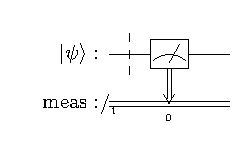
\includegraphics[width=0.2\textwidth]{figs/measure_z.pdf}
                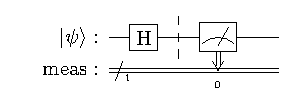
\includegraphics[width=0.325\textwidth]{figs/measure_x.pdf}
                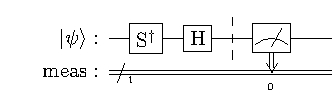
\includegraphics[width=0.325\textwidth]{figs/measure_y.pdf}
            \end{center}
            \caption{Mesures des observables $Z$, $X$ et $Y$ respectivement. L'état
            représenté est un état quelconque à un seul qubit. Pour plusieurs qubits,
            il suffit d'appliquer le changement de base à chacun avant la mesure.}
            \label{fig:mes}
        \end{figure}
        Dans le cas présent, l'hamiltonien se décompose en chaines de Pauli de la
        manière suivante.
        \begin{align}
            H&=t\sum_{<i,j>}\mathbf{S}_i\cdot\mathbf{S}_j\\
            &=t\sum_{<i,j>}\qty(S_{xi}S_{xj}+S_{yi}S_{yj}+S_{zi}S_{zj})
        \end{align}
        Laissant donc trois familles de chaines de Pauli, ayant chacune seulement
        deux qubits à mesurer. On peut généraliser le raisonnement précédent pour
        obtenir la valeur moyenne d'un opérateur étant le produit tensoriel de
        deux fois la même matrice de Pauli, en regardant les éléments de matrice
        d'une telle chaine.
        \begin{align}
            \expval{\sigma_i\sigma_j}_B&=\frac{\nu_{0iB}^{0j}+\nu_{1iB}^{1i}-\nu_{0iB}^{1j}-\nu_{1iB}^{0j}}{N_{\text{shots}}}
        \end{align}
        où $i$ et $j$ sont les indices du réseau. Les $\nu^{mj}_{niB}$ représentent le nombre
        de mesures dans la base $B$ ayant obtenue $m$ pour le $j$ ième qubit et $n$ pour le $i$ ième
        qubit.\\
        Le coeur du problème se situe dans l'état d'essai. Un état d'essai
        parfait aurait un domaine de paramètre permettant d'atteindre le vrai
        minimum d'énergie, tout en ayant très peu de paramètres libres de varier.
        Or, tel que mentionné, un état général pour un réseau à $12$ spins
        possède $2^{12}$ degrés de liberté. Il s'agit alors d'un effort de
        modélisation qui permet de trouver le meilleur état d'essai. La technique
        utilisée dans ce travail sera de se pencher sur la physique du problème
        afin de cerner les meilleurs degrés de liberté à considérer. Tout d'abord,
        étant donné que l'on s'attend à un liquide de spin comme état fondamental,
        il faut que ceux-ci puissent avoir n'importe quelle orientation, tant
        que les voisins les plus proches sont anti-alignés. Pour cette raison,
        l'état d'essai à privilégier devra favoriser cette caractéristique.
        Pour y arriver, $2$ états d'essai ont été conçu avec cette idée en tête.\\
        Le premier état d'essai à considérer est très simple, avec $24$ paramètres
        libres.
        \begin{figure}[H]
            \begin{center}
                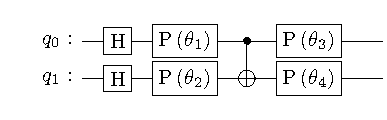
\includegraphics[width=0.95\textwidth]{figs/ansatz1.pdf}
            \end{center}
            \caption{Bloc de circuit préparant le premier état d'essai. Ce bloc est
            répété entre chaque qubits présentant un lien dans le réseau. Les deux
            qubits représentés sont ceux pour lesquels un lien existe sur le réseau,
            il n'y aurait pas de porte $CX$ entre deux site pour lesquels il n'y a
            pas de lien.}
            \label{fig:}
        \end{figure}
        Les paramètres libre de ce circuit contrôles les phases individuelles
        de chaque qubit avant et après le terme d'interaction, représenté par
        la porte $CX$. Ceci permet d'approcher le minimum car cet état permet
        la minimisation du terme en chaine de Pauli contenant des matrices $XX$.
        En effet, avec les bons paramètres, il est possible de sélectionner
        seulement des états pour lesquels les valeurs moyennes des matrices $XX$
        sont négatifs. Ces mêmes états donnent des valeurs moyennes nulles pour
        les autres chaines de Pauli, contenant les $YY$ et les $ZZ$.\\
        Le second état d'essai à considérer apporte cette idée plus loin. Avec
        $2$ fois plus de paramètres, on peut ajouter une inclinaison par rapport
        au plan $O_{xy}$, sur la sphère de Bloch, supplémentaire aux qubits.
        \begin{figure}[H]
            \begin{center}
                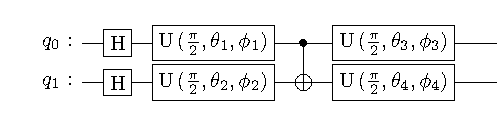
\includegraphics[width=0.95\textwidth]{figs/ansatz2.pdf}
            \end{center}
            \label{fig:}
        \end{figure}
        En considérant seulement deux qubits, ces paramètres permettent entièrement
        de minimiser les observables $ZZ$, $XX$ et $YY$ en même temps. Dans le cas
        à l'étude ici, ce n'est pas le cas car les paramètres qui minimisent
        individuellement chaque observables ne sont pas les mêmes. Ces deux états
        d'essai ont un problème important, soit le fait qu'ils sont dépendant
        de l'ordre d'itération sur le réseau. En effet, selon l'ordre d'application
        des termes d'interaction, l'état obtenu ne sera pas le même. Il s'agit
        d'une symétrie qu'on s'attendrait à retrouver dans l'état fondamental, comme
        tous les liens ont le même poids dans le calcul de l'énergie du fondamental.


    % subsubsection Variationnal Quantum Eigensolver (VQE)} (end)


    % section Méthode (end)

\clearpage
\end{document}
